\documentclass[
  bibliography=totoc,     % Literatur im Inhaltsverzeichnis
  captions=tableheading,  % Tabellenüberschriften
  titlepage=firstiscover, % Titelseite ist Deckblatt
]{scrartcl}

% Paket float verbessern
\usepackage{scrhack}

% Warnung, falls nochmal kompiliert werden muss
\usepackage[aux]{rerunfilecheck}

% unverzichtbare Mathe-Befehle
\usepackage{amsmath}
% viele Mathe-Symbole
\usepackage{amssymb}
% Erweiterungen für amsmath
\usepackage{mathtools}

% Fonteinstellungen
\usepackage{fontspec}
% Latin Modern Fonts werden automatisch geladen
% Alternativ:
%\setromanfont{Libertinus Serif}
%\setsansfont{Libertinus Sans}
%\setmonofont{Libertinus Mono}
\recalctypearea % Wenn man andere Schriftarten gesetzt hat,
% sollte man das Seiten-Layout neu berechnen lassen

% deutsche Spracheinstellungen
\usepackage{polyglossia}
\setmainlanguage{german}


\usepackage[
  math-style=ISO,    % ┐
  bold-style=ISO,    % │
  sans-style=italic, % │ ISO-Standard folgen
  nabla=upright,     % │
  partial=upright,   % ┘
  warnings-off={           % ┐
    mathtools-colon,       % │ unnötige Warnungen ausschalten
    mathtools-overbracket, % │
},                       % ┘
]{unicode-math}

% traditionelle Fonts für Mathematik
\setmathfont{Latin Modern Math}
% Alternativ:
%\setmathfont{Libertinus Math}

\setmathfont{XITS Math}[range={scr, bfscr}]
\setmathfont{XITS Math}[range={cal, bfcal}, StylisticSet=1]

% Zahlen und Einheiten
\usepackage[
locale=DE,                   % deutsche Einstellungen
separate-uncertainty=true,   % immer Fehler mit \pm
per-mode=symbol-or-fraction, % / in inline math, fraction in display math
]{siunitx}

% chemische Formeln
\usepackage[
version=4,
math-greek=default, % ┐ mit unicode-math zusammenarbeiten
text-greek=default, % ┘
]{mhchem}

% richtige Anführungszeichen
\usepackage[autostyle]{csquotes}

% schöne Brüche im Text
\usepackage{xfrac}

% Standardplatzierung für Floats einstellen
\usepackage{float}
\floatplacement{figure}{htbp}
\floatplacement{table}{htbp}

% Floats innerhalb einer Section halten
\usepackage[
section, % Floats innerhalb der Section halten
below,   % unterhalb der Section aber auf der selben Seite ist ok
]{placeins}

% Seite drehen für breite Tabellen: landscape Umgebung
\usepackage{pdflscape}

% Captions schöner machen.
\usepackage[
  labelfont=bf,        % Tabelle x: Abbildung y: ist jetzt fett
  font=small,          % Schrift etwas kleiner als Dokument
  width=0.9\textwidth, % maximale Breite einer Caption schmaler
]{caption}
% subfigure, subtable, subref
\usepackage{subcaption}

% Grafiken können eingebunden werden
\usepackage{graphicx}
% größere Variation von Dateinamen möglich
\usepackage{grffile}

% schöne Tabellen
\usepackage{booktabs}

% Verbesserungen am Schriftbild
\usepackage{microtype}

% Literaturverzeichnis
\usepackage[style=alphabetic,]{biblatex}
% Quellendatenbank
\addbibresource{lit.bib}

% Hyperlinks im Dokument
\usepackage[
  unicode,        % Unicode in PDF-Attributen erlauben
  pdfusetitle,    % Titel, Autoren und Datum als PDF-Attribute
  pdfcreator={},  % ┐ PDF-Attribute säubern
  pdfproducer={}, % ┘
]{hyperref}
% erweiterte Bookmarks im PDF
\usepackage{bookmark}

% Trennung von Wörtern mit Strichen
\usepackage[shortcuts]{extdash}

\title{V103: Biegung elastischer Stäbe}
\author{
  Simon Schulte
  \texorpdfstring{
    \\
    \href{mailto:simon.schulte@udo.edu}{simon.schulte@udo.edu}
  }{}
  \texorpdfstring{\and}{, }
  Tim Sedlaczek
  \texorpdfstring{
    \\
    \href{mailto:tim.sedlaczek@udo.edu}{tim.sedlaczek@udo.edu}
  }{}
}
\publishers{TU Dortmund – Fakultät Physik}

\date{Durchführung: 22.12.2016\\
      Abgabe: 10.01.2016}


\begin{document}

\maketitle
\thispagestyle{empty}
\tableofcontents
\newpage
\section{Zielsetzung}
\label{sec:zielsetzung}
Ziel des Versuchs ist die Bestimmung des Elastizitätsmodules $E$ verschiedener
Metalle über die Untersuchung der Durchbiegung $D$ eingespannter metallischer Stäbe.
\section{Theorie}
\label{sec:theorie}
Wenn auf einen eingespannten Festkörper eine Kraft wirkt, verformt sich dieser.
Diese Änderung kann als Volumenänderung oder als Gestaltsänderung vorliegen.
Es ist von der sogenannten Spannung $\sigma$ abhängig, ob ein Festkörper
unter Einwirkung von Kräften eine Volumen- oder Gestaltsänderung erfährt.
$\sigma$ ist als Kraft pro Fläche definiert. Die Spannung $\sigma$ wirkt in
Normalrichtung der angegriffenen Fläche des Körpers und ist über das Hooksche
Gesetz durch
\begin{equation}
	\sigma=E\,\frac{\mathup{\Delta}L}{L}
	\label{eq:spannung}
\end{equation}
definiert. Dabei ist $E$ der Elastizitätsmodul. Damit gibt die Spannung $\sigma$
an, wie stark die am Körper wirkende Spannung bei einer relativen Änderung einer
linearen Körperdimension ausfällt. Dieser Zusammenhang ist in dem sogenannten
Hookschen Bereich linear. Vergleichbar mit der Kleinwinkelnäherung ist der
Hooksche Bereich in einem Bereich kleiner Auslenkungen definiert. Durch die
Bestimmung der Längenänderung $\mathup{\Delta}L$ bei einer bekannten Kraft
kann somit der Elastizitätsmodul $E$ bestimmt werden. Bei der Messung der Biegung
$D$ treten bei gleichen Kraftverhältnissen und Abmessungen des Versuchsaufbaus
deutlich größere und genauer zu bestimmende Werte auf. $D$ ist deutlich besser
und genauer zu bestimmen, als der Elastizitätsmodul $E$. Es gilt allerdings bei
der Biegung elastischer Metallstäbe zwei Fälle zu unterscheiden.
\subsection{Biegung des einseitig eingespannten homogenen Stabes}
\begin{figure}[H]
    \centering
    \caption{Schematische Darstellung der Durchbiegung bei einseitiger Einspannung. \cite{anleitung}}
    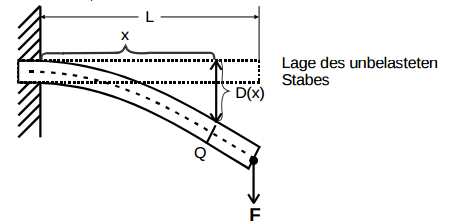
\includegraphics[width=0.75\textwidth]{V1031.png}
    \label{fig:1031}
\end{figure}
In Abbildung \ref{fig:1031} dargestellt ist ein einseitig fest eingespannter,
homogener Stab, auf den eine Kraft $F$ am freien Ende wirkt. Dann biegt sich
dieser Stab durch. Durch diese Durchbiegung erfährt der Stab eine
kontinuierliche Längenänderung $\delta{L}$, welche widerum über den Querschnitt
$Q$, des jeweiligen Metallstabs, der gerade eingespannt ist, variiert. $D(x)$
ist die Durchbiegung des Stabs. Das darin enthaltene $x$ gibt die Strecke von
dem Ort, an dem der Stab eingespannt ist, bis zu dem Ort, an dem die
Durchbiegung gemessen wird, an. Wenn man sich den Metallstab als Stab, welcher
aus vielen "Metallfasern" besteht vorstellt, dann folgt: Fasern, die weiter oben
liegen werden gestreckt und somit auseinandergezogen. Fasern, die unterhalb der
längeninvarianten neutralen Faser liegen, also jene, die in \ref{fig:1031}
gestrichelt mitten durch den Metallstab geht, werden gestaucht, also verkürzt.
Die neutrale Faser bahält immer ihre Ausgangslänge. Durch die wirkende
Kraft $F$ am Ende des Stabes folgt ein Drehmoment $M_f$ mit Hebelarm $(L-x)$,
was die zuvor beschriebene Verbiegung zur Folge hat. Es wirkt dabei mit
entgegengesetzter Richtung ein Drehmoment $M_\sigma$ entgegen, welches aus der
Elastizität des jeweiligen Stoffes, aus dem der Metallstab besteht, folgt. Die
messbare Auslenkung des Stabes charakterisiert also das Gleichgewicht dieser
Drehmomente, für das

\begin{align}
	M_f&=M_\sigma\\
	F(L-x)&=\int_Q y\sigma(y)\mathup{d}q
\end{align}

gilt. Das Gleichgewicht wird also von der hebelnden Kraft und der Spannung
charakterisiert. Die Gleichung \eqref{eq:spann} lässt sich mit Hilfe der
Beziehung

\begin{equation}
	\frac{1}{R}\approx\frac{\mathup{d}^2D}{\mathup{d}x^2}
	\label{eq:approx}
\end{equation}

aus der Differentialgeometrie vereinfachen. Daraus folgt mit Definition des
Flächenträgheitsmomentes $I$ als

\begin{equation}
	I:=\int_Q y^2 \mathup{d}q(y)
	\label{eq:trägheit}
\end{equation}

für die Durchbiegung auf der Länge $L$ des Stabes die Gleichung

\begin{equation}
	D(x)=\frac{F}{2EI}\left(Lx^2-\frac{x^3}{3}\right)\text{.}
	\label{eq:durchbieg}
\end{equation}

\subsection{Biegung des beidseitig eingespannten homogenen Stabes}
\begin{figure}[H]
    \centering
    \caption{Schematische Darstellung der Durchbiegung bei zweiseitiger Einspannung. \cite{anleitung}}
    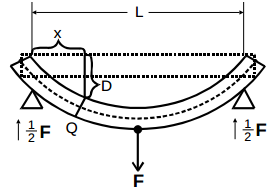
\includegraphics[width=0.75\textwidth]{V1032.png}
    \label{fig:1032}
\end{figure}
In Abbildung \ref{fig:1032} dargestellt ist ein beidseitig eingespannter Stab.
Hier wirkt nun mittig auf den Stab die Kraft $F$. Durch diese wirkende Kraft $F$
ergibt sich auch hier jeweils ein Drehmoment auf beiden Seiten der Auslenkung.
Links von der Auslenkung ergibt sich folgendes Drehmoment:
\begin{equation}
	M_F=-\frac{F}{2}x, \;\;\; 0\leqslant  x\leqslant\frac{L}{2}\text{,}
\label{eq:Drehmoment_links}
\end{equation}
Rechts von der Auslenkung ergibt sich folgendes Drehmoment:
\begin{equation}
	M_F=-\frac{F}{2}(L-x), \;\;\; \frac{L}{2}\leqslant  x\leqslant L
\end{equation}
Aus diesen beiden Gleichungen ist es möglich, mit dem gleichen Ansatz, wie bei
der einseitigen Einspannung, zwei Differentialgleichungen dür die Durchbiegung
zu bestimmen.
\begin{align}
	\frac{\mathup{d}^2D}{\mathup{d}x^2}&=-\frac{F\cdot x}{2EI}, \;\;\; 0\leqslant x\leqslant\frac{L}{2}\text{,}
    \label{eq:dgl_beidseitig1} \\
	\frac{\mathup{d}^2D}{\mathup{d}x^2}&=-\frac{F}{2EI}(L-x), \;\;\; \frac{L}{2}\leqslant x\leqslant L
	\label{eq:dgl_beidseitig}
\end{align}
Mit zweifacher Integration der Gleichungen \eqref{eq:dgl_beidseitig1} und
\eqref{eq:dgl_beidseitig} ergibt sich für die Durchbiegung $D$:
\begin{align}
	D(x)&=\frac{F}{48EI}(3L^2x-4x^3), \;\;\; 0\leqslant  x\leqslant\frac{L}{2}\text{,}
    \label{eq:gl_Biegung1} \\
	D(x)&=\frac{F}{48EI}(4x^3-12Lx^2+9L^2x-L^3), \;\;\; \frac{L}{2}\leqslant  x\leqslant L
	\label{eq:gl_Biegung}
\end{align}
Allerdings nur unter der Bedingung, dass die Stabmitte, also der Ort, an dem die
Kraft angreift, eine horizontale Tangente aufweist. Außerdem muss die Durchbiegung
an beiden Auflagepunkten gleich Null sein. Mit den beiden Gleichungen
\eqref{eq:gl_Biegung} und \eqref{eq:gl_Biegung1} kann man durch Herleiten eines
Zusammenhanges von $D$ und $x$ aus den gemessenen Messwerten der
Elastizitätsmodul $E$ berechnen.
\newpage
\section{Durchführung}
\label{sec:durchführung}
\begin{figure}[H]
    \centering
    \caption{Schematische Darstellung der Messapparatur. \cite{anleitung}}
    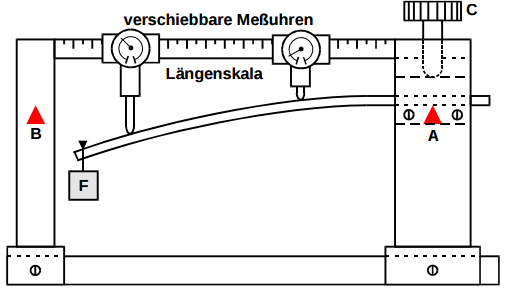
\includegraphics[width=0.75\textwidth]{V1033.png}
    \label{fig:1033}
\end{figure}
In Abbildung \ref{fig:1033} zu sehen ist der Versuchsaufbau, der zur Messung
verwendet wird. Die Durchbiegung $D$ wird mit verschiebbaren Messuhren gemessen.
Diese messen extrem genau, mit Hilfe eines federnden Taststiftes, Verschiebungen
eines Objekts. Verschiebbar sind sie, um die Durchbiegung $D$ an verschiedenen
Orten $x$ messen zu können. Die Messuhren befinden sich auf einer festen Achse.
Sie besitzen zur Messung ausfahrbare Auflagepunkte zur Bestimmung des Abstandes
von einem kalibrieten Nullpunkt in einem Wertebereich von $0,01$ bis $\SI{10}{\milli\meter}$.
Der Stab kann sowohl an einer Seite, wie auch in der Abbildung \ref{fig:1033}
dargestellt, eingespannt sein, als auch an zwei Seiten. Dann wird der Stab etwa
dort eingespannt, wo sich in der Abbildung "B" befindet.
Nun werden zuerst die Versuchsparameter aufgenommen. Das sind der Durchmesser
$d$, die effektive Länge $L$ und das Gewicht der drei Stäbe, die untersucht
werden. Das sind zum einen ein eckiger Aluminiumstab, außerdem ein runder
Aluminiumtab und ein eckiger Messingstab. $L$ und das Gewicht des jeweiligen
Stabes werden einmal gemessen und der Durchmesser $d$ wird für jeden Stab 5 mal
gemessen.
\subsection{Einseitige Einspannung}
Als nächstes werden zwei verschiede Stäbe in einseitiger Einspannung untersucht,
zum einen der eckige Messingstab und zum anderen der runde Aluminumstab.
Dazu wird der jeweilige Stab an der rechten Seite in einen Klemmblock gespannt,
in Abbildung \ref{fig:1033} zu sehen. Nun wird die Messuhr von rechts an die
Probe gesetzt und kalibriert. Dafür werden solange Veränderungen an verschiedenen
Stellen der Messuhr vorgenommen, bis die mit am Ende der Probe angehängten
Gewicht gemessene Durchbiegung bei minimaler Auslenkung auf der Längenskala
gerade Null beträgt. Dann werden in $1,5cm$ Schritten Werte aufgenommen. Dafür
wird die Masse angehängt und mit der Messuhr langsam der Stab abgefahren.
\subsection{Beidseitige Einspannung}
Als letztes wird der beidseitig eingespannte eckige Aluminiumstab untersucht.
Dafür wird nun der Stab auf der anderen Seite ebenfalls eingespannt. Dann wird
zuerst, analog, wie bei der einseitigen Einspannung, ohne ein zusätzliches
Massestück die Durchbiegung $D$ abhägig vom Ort $x$ gemessen. Danach wird eine
Masse angehangen und die Messung wird erneut analog, wie bei der einseitigen
Einspannung durchgeführt.
\newpage
\section{Fehlerrechnung}
\label{sec:fehlerrechnung}
Die in der Auswertung verwendeten Mittelwerte mehrfach gemessener Größen sind
gemäß der Gleichung
\begin{equation}
    \bar{x}=\frac{1}{n}\sum_{i=1}^n x_i.
    \label{eq:mittelwert}
\end{equation}

bestimmt. Die Standardabweichung des Mittelwertes ergibt sich dabei zu

\begin{equation}
    \mathup{\Delta}\bar{x}=\sqrt{\frac{1}{n(n-1)}\sum_{i=1}^n\left(x_i-\bar{x}\right)^2}.
    \label{eq:standardabweichung}
\end{equation}

Resultiert eine Größe über eine Gleichung aus zwei anderen fehlerbehafteten
Größen, so berechnet sich der Gesamtfehler nach der Gaußschen
Fehlerfortpflanzung zu

\begin{equation}
    \mathup{\Delta}f(x_1,x_2,...,x_n)=\sqrt{\left(\frac{\mathup{d}f}{\mathup{d}x_1}\mathup{\Delta}x_1\right)^2+\left(\frac{\mathup{d}f}{\mathup{d}x_2}\mathup{\Delta}x_2\right)^2+ \dotsb +\left(\frac{\mathup{d}f}{\mathup{d}x_n}\mathup{\Delta}x_n\right)^2}.
\end{equation}

Alle in der Auswertung angegebenen Größen sind stets auf die erste signifikante
Stelle des Fehlers gerundet. Setzt sich eine Größe über mehrere Schritte aus
anderen Größen zusammen, so wird erst am Ende gerundet, um Fehler zu vermeiden.
Zur Auswertung wurde das Programm \texttt{python (Version 3.5.2)} verwendet.
\newpage
\section{Auswertung}
\label{sec:auswertung}
\subsection{Berechnung des Elastizitätsmoduls $E$ eines Messingstabes mit quadratischem Querschnitt bei einseitiger Einspannung}
In der Tabelle \ref{tab:messing} zu sehen sind die Versuchsparameter des
Messingstabes. Die Werte werden, wie in \ref{sec:durchführung} beschrieben,
bestimmt. Eine Fehlerrechnung für den Durchmesser des Messingstabes bleibt aus,
da sich höchtens Abweichungen von wenigen Mikrometern bei den 5 Messungen ergeben.
\begin{table}[H]
    \centering
    \caption{Versuchsparameter für den Messingstab.}
    \begin{tabular}{lS}
        \toprule
        Durchmesser $d$      & \SI{10}{\milli\metre}   \\
        effektive Länge $L$  & \SI{40.7}{\centi\metre} \\
        angehängte Masse $M$ & \SI{2.3606}{\kilo\gram} \\
        \bottomrule
    \end{tabular}
    \label{tab:messing}
\end{table}
Das Flächenträgheitsmoment des Messingstabes ergibt sich mit
\begin{equation}
    I = \frac{d^4}{12} = \SI{833}{\milli\metre^4}.
\end{equation}
Tabelle \ref{tab2:messing} beinhaltet die gemessene effektive Auslenkung des
Stabes in Abhängigkeit der Entfernung vom Einspannungspunkt.
\begin{table}[H]
    \centering
    \caption{Effektive Durchbiegung des einseitig eingespannten Messingstabes in Abhängigkeit des Ortes mit angehängter Masse.}
    \begin{tabular}{cc}
        \toprule
        {Ort} & {Auslenkung} \\
        {$x[\si{\centi\metre}]$} & {$D[\si{\micro\metre}]$} \\
        \midrule
         3,0 &    0 \\
         4,5 &    2 \\
         6,0 &    7 \\
         7,5 &  7,5 \\
         9,0 &    0 \\
        10,5 &   -2 \\
        12,0 &  -14 \\
        13,5 &  -24 \\
        15,0 &  -29 \\
        16,5 &  -40 \\
        18,0 &  -56 \\
        19,5 &-73,5 \\
        21,0 &  -88 \\
        22,5 & -116 \\
        24,0 & -132 \\
        25,5 & -153 \\
        27,0 & -175 \\
        28,5 & -195 \\
        30,0 & -221 \\
        31,5 & -242 \\
        33,0 & -266 \\
        \bottomrule
    \end{tabular}
    \label{tab2:messing}
\end{table}
Zur Berechnung des Elastizitätsmoduls $E$ muss nun die effektive Auslenkung des
Stabes nach unten in Abhängigkeit des Hebelarms betrachtet werden wenn, mit der
Masse $M$ an das freie Ende des Stabes gehangen. In Tabelle~\ref{tab2:messing}
zu sehen sind die aufgenommenen Messwerte, wobei die Auslenkung $D$ des Stabes
bereits um die Auslenkung bereinigt wurde, die der Stab aufgrund seines Eigengewichtes
selbst verursacht.

In einem weiteren Schritt wird nun gemäß Gleichung \eqref{eq:durchbieg} eine
lineare Regression der Messwerte vorgenommen.

Die lineare Ausgleichsrechnung, welche auf der Gleichung \eqref{eq:durchbieg}
basiert, liefert für die Steigung $m$ und den y-Achsenabschnitt $b$ die Werte:
\begin{align}
    m &= \SI{-0.0087(2)}{\frac{1}{\metre\squared}} \\
    b &= \SI{0.000028(4)}{\metre}.
\end{align}
Für den Elastizitätsmodul $E$ folgt mit der Formel
\begin{equation}
    E = \frac{F}{2mI} = \frac{Mg}{2mI} = \SI{1589(44)}{\kilo\newton\per\milli\metre\squared}.
    \label{eq:E}
\end{equation}
\subsection{Berechnung des Elastizitätsmoduls $E$ eines Aluminiumstabes mit kreisförmigem Querschnitt bei einseitiger Einspannung}
In der Tabelle \ref{tab:alurund} zu sehen sind die Versuchsparameter des
Messingstabes. Die Werte werden wie in \ref{sec:durchführung} beschrieben
bestimmt. Eine Fehlerrechnung für den Durchmesser des kreisförmigen
Aluminiumstabes bleibt aus, da sich höchtens Abweichungen von wenigen
Mikrometern bei den 5 Messungen ergeben.
\begin{table}[H]
    \centering
    \caption{Versuchsparameter für den runden Aluminiumstab.}
    \begin{tabular}{lS}
        \toprule
        Durchmesser $d$      & \SI{10}{\milli\metre}   \\
        effektive Länge $L$  & \SI{34.8}{\centi\metre} \\
        angehängte Masse $M$ & \SI{1.19296}{\kilo\gram} \\
        \bottomrule
    \end{tabular}
    \label{tab:alurund}
\end{table}
Das Flächenträgheitsmoment des runden Aluminiumstabes ist mit Gleichung
\eqref{eq:trägheit}:
\begin{equation}
    I = \frac{\pi}{64}d^4 = \SI{491}{\milli\metre^4}
\end{equation}
Die lineare Ausgleichsrechnung liefert für die Ausgleichsgerade die Parameter
\begin{align}
    m &= \SI{-0.02101(3)}{\frac{1}{\metre\squared}} \\
    b &= \SI{0.00020(4)}{\metre}.
\end{align}
\begin{table}[H]
    \centering
    \caption{Effektive Durchbiegung des einseitig eingespannten runden Alustabes in Abhängigkeit des Ortes mit angehängtem Gewicht.}
    \begin{tabular}{cc}
        \toprule
        {Ort} & {Auslenkung} \\
        {$x[\si{\centi\metre}]$} & {$D[\si{\micro\metre}]$} \\
        \midrule
         2,5 &  -16 \\
         4,0 &    3 \\
         5,5 &   -8 \\
         7,0 &  -11 \\
         8,5 &  -32 \\
        10,0 &  -44 \\
        11,5 &  -64 \\
        13,0 &  -89 \\
        14,5 & -102 \\
        16,0 &-125,5\\
        17,5 &-157,5\\
        19,0 & -190 \\
        20,5 &-216,5\\
        22,0 & -256 \\
        23,5 & -284 \\
        25,0 &-317,5\\
        26,5 &-350,8\\
        28,0 &-406,5\\
        29,5 &-445.5\\
        31,0 & -484 \\
        32,5 & -529 \\
        \bottomrule
    \end{tabular}
    \label{tab2:alurund}
\end{table}
Für den Elastiziätsmodul folgt dann mit der Formel \ref{eq:E}
\begin{equation}
    E = \frac{F}{2mI} = \frac{Mg}{2mI} = \SI{566(8)}{\kilo\newton\per\milli\metre\squared}.
\end{equation}
\subsection{Berechnung des Elastizitätsmoduls $E$ eines Aluminiumstabes mit quadratischem Querschnitt bie beidseitiger Einspannung}
In der Tabelle \ref{tab:alueckig} zu sehen sind die Versuchsparameter des
Messingstabes. Die Werte werden wie in \ref{sec:durchführung} beschrieben
bestimmt. Eine Fehlerrechnung für den Durchmesser des eckigen Aluminiumstabes
bleibt aus, da sich höchtens Abweichungen von wenigen Mikrometern bei den 5
Messungen ergeben.
\begin{table}[H]
    \centering
    \caption{Versuchsparameter für den eckigen Aluminiumstab.}
    \begin{tabular}{lS}
        \toprule
        Durchmesser $d$      & \SI{10}{\milli\metre}   \\
        effektive Länge $L$  & \SI{55.2}{\centi\metre} \\
        angehängte Masse $M$ & \SI{3.5312}{\kilo\gram} \\
        \bottomrule
    \end{tabular}
    \label{tab:alueckig}
\end{table}
\begin{table}[H]
    \centering
    \caption{Effektive Durchbiegung des beidseitig eingespannten eckigen Alustabes in Abhängigkeit des Ortes.}
    \begin{tabular}{cc}
        \toprule
        {Ort} & {Auslenkung} \\
        {$x[\si{\centi\metre}]$} & {$D[\si{\micro\metre}]$} \\
        \midrule
         2,5 &    0 \\
         4,0 & 10,0 \\
         5,5 & 23,0 \\
         7,0 & 33,5 \\
         8,5 & 43,5 \\
        10,0 & 54,0 \\
        11,5 & 60,5 \\
        13,0 & 71,5 \\
        14,5 & 83,5 \\
        16,0 & 87,0 \\
        17,5 & 93,0 \\
        19,0 & 95,0 \\
        20,5 & 95,5 \\
        22,0 & 95,5 \\
        23,5 &  105 \\
        25,0 &  107 \\
        30,0 & 83,0 \\
        34,0 & 95,5 \\
        38,0 & 96,0 \\
        42,0 & 86,5 \\
        46,0 & 55,2 \\
        50,0 & 33,0 \\
        54,0 & 11,0 \\
        \bottomrule
    \end{tabular}
    \label{tab2:alueckig}
\end{table}
\begin{table}[H]
    \centering
    \caption{Effektive Durchbiegung des beidseitig eingespannten eckigen Alustabes in Abhängigkeit des Ortes mit angehängter Masse.}
    \begin{tabular}{cc}
        \toprule
        {Ort} & {Auslenkung} \\
        {$x[\si{\centi\metre}]$} & {$D[\si{\micro\metre}]$} \\
        \midrule
      2,5   & -3,0  \\
      4,0   &  2,5  \\
      5,5   &  13,5 \\
      7,0   &  18,0 \\
      8,5   & 22.0 \\
      10,0  & 23,0 \\
      11,5  & 26,0 \\
      13,0  & 27,0 \\
      14,5  & 36,0 \\
      16,0  & 36,0 \\
      17,5  & 34,5 \\
      19,0  & 28,0 \\
      20,5  & 30,5 \\
      22,0  & 24,0 \\
      23,5  & 28,0 \\
      25,0  & 29,5 \\
      30,0  &-11,0 \\
      34,0  & 8,0  \\
      38,0  & 21,0 \\
      42,0  & 25,5 \\
      46,0  & 16,0 \\
      50,0  & 12,5 \\
      54,0  & 10,0 \\
        \bottomrule
    \end{tabular}
    \label{tab3:alueckig}
\end{table}
Bei der Regression der Messwerte muss beachtet werden, dass für die beidseitige
Auflage des Stabes nun  verschiedene Gleichungen verwendet werden müssen, um die
$x$-Werte in Bezug auf die Auslenkung $D$ zu linearisieren. Insbesondere gilt
für den Abschnitt $0\leqslant x\leqslant\sfrac{L}{2}$ eine andere Beziehung als
für den Abschnitt $\sfrac{L}{2}\leqslant x\leqslant L$. Die entsprechenden
Gleichungen~\eqref{eq:gl_Biegung1} und~\eqref{eq:gl_Biegung} sind im Theorieteil
angegeben.

Die lineare Regression im Bereich $0\leqslant x\leqslant\sfrac{L}{2}$ liefert die Parameter

\begin{align}
    m_1 &= \SI{0.00028(3)}{\frac{1}{\metre\squared}} \\
    b_1 &= \SI{-0.00003(4)}{\metre}.
\end{align}


Der Zusammenhang mit dem Elastizitätsmodul $E$ folgt aus Gleichung~\eqref{eq:gl_Biegung1}. Hierbei ist
erneut die in der Ausgleichsrechnung ermittelte Steigung $m$ über das Flächenträgheitsmoment $I$ und das
Gewicht $M$ der angehängten Masse mit $E$ verbunden.

\begin{equation}
    m = \frac{F}{48EI}
\end{equation}

Durch Umformung folgt für den Elastizitätsmodul

\begin{equation}
    E_1 = \frac{F}{48mI} = \frac{Mg}{48mI} = \SI{3073(388)}{\kilo\newton\per\milli\metre\squared}.
\end{equation}

Die Bestimmung des Elastizitätsmoduls für den Abschnitt $\sfrac{L}{2}\leqslant x\leqslant L$ erfolgt
analog, mit dem Unterschied, dass nun Gleichung~\eqref{eq:dgl_beidseitig} für die lineare Regression
genutzt wird. Für Steigung und y-Achsenabschnitt ergibt sich

\begin{align}
    m_2 &= \SI{0.00041(8)}{\frac{1}{\metre\squared}} \\
    b_2 &= \SI{0.00013(1)}{\metre}.
\end{align}

Daraus folgt der Elastizitätsmodul

\begin{equation}
    E_2 = \frac{Mg}{48mI} = \SI{20851(38082)}{\kilo\newton\per\milli\metre\squared}.
\end{equation}

Abschließend werden die beiden Werte $E_1$ und $E_2$ gemittelt, sodass sich für den Elastizitätsmodul $E$
von Stahl der Wert

\begin{equation}
    E = \SI{11962(19042)}{\kilo\newton\per\milli\metre\squared}.
\end{equation}

ergibt.
\newpage
\section{Diskussion}
\label{sec:diskussion}
Nun werden die ermittelten Werte für den ermittelten Elastizitätsmodul der drei
verschiedenen Proben mit Literaturwerten verglichen. In Tabelle \ref{tab:ergebnisse}
zu sehen ist der Vergleich der ermittelten Werte mit den Literaturwerten,
inklusive der jeweiligen Abweichung.
\begin{table}[h]
    \centering
    \caption{Ergebnisse zur Bestimmung des Elastizitätsmoduls verschiedener Proben.}
    \begin{tabular}{lccc}
        \toprule
        & {Experimenteller Wert} & {Literaturwert \cite{chemie}} & {Abweichung} \\
        & in $\si{\kilo\newton\per\milli\metre\squared}$ & in $\si{\kilo\newton\per\milli\metre\squared}$ & in $\si{\percent}$ \\
        \midrule
        Messing   & 1589 \pm\,44 & 78-123     &  1500 \\
        Alu rund  & 566 \pm\,8     & 70 & 808 \\
        Alu eckig & 11962 \pm\,19042    & 70   & 0\\
        \bottomrule
    \end{tabular}
    \label{tab:ergebnisse}
\end{table}\\
Die Ergebnisse weichen unterschiedlich stark von den Literaturwerten ab. Für den
runden Messingstab ergibt sich eine Abweichung von etwa $\SI{1500}{\percent}$,
für den runden Alustab eine Abweichung von etwa $\SI{808}{\percent}$ und der
eckige Alustab hat einen größeren Fehler, als den Messwert selbst. Unter
Einbeziehung des Fehlers kann man theoretisch sagen, dass der Fehler
$\SI{0}{\percent}$ groß ist. Allerdings ist dieser Wert nicht repräsentativ.
Die Abweichungen der anderen Elastizitätsmodule sind ebenfalls sehr groß.
Daraus folgt, dass die vorliegenden Messwerte nicht gut sind. Das wird vorallem
daran liegen, dass die Messuhren sehr wackelig waren. Es war kaum möglich diese
zu Nullen. Wenn testweise die Messuhren richtig kalibriert wurden und man einmal
den Stab abgefahren ist und wieder zurück, war diese danach nicht mehr richtig
kalibriert. Insgesamt sind die vorliegenden Messwerte nicht repräsentativ.
\nocite{*}
\printbibliography
\section{Anhang}
\begin{figure}[H]
    \centering
    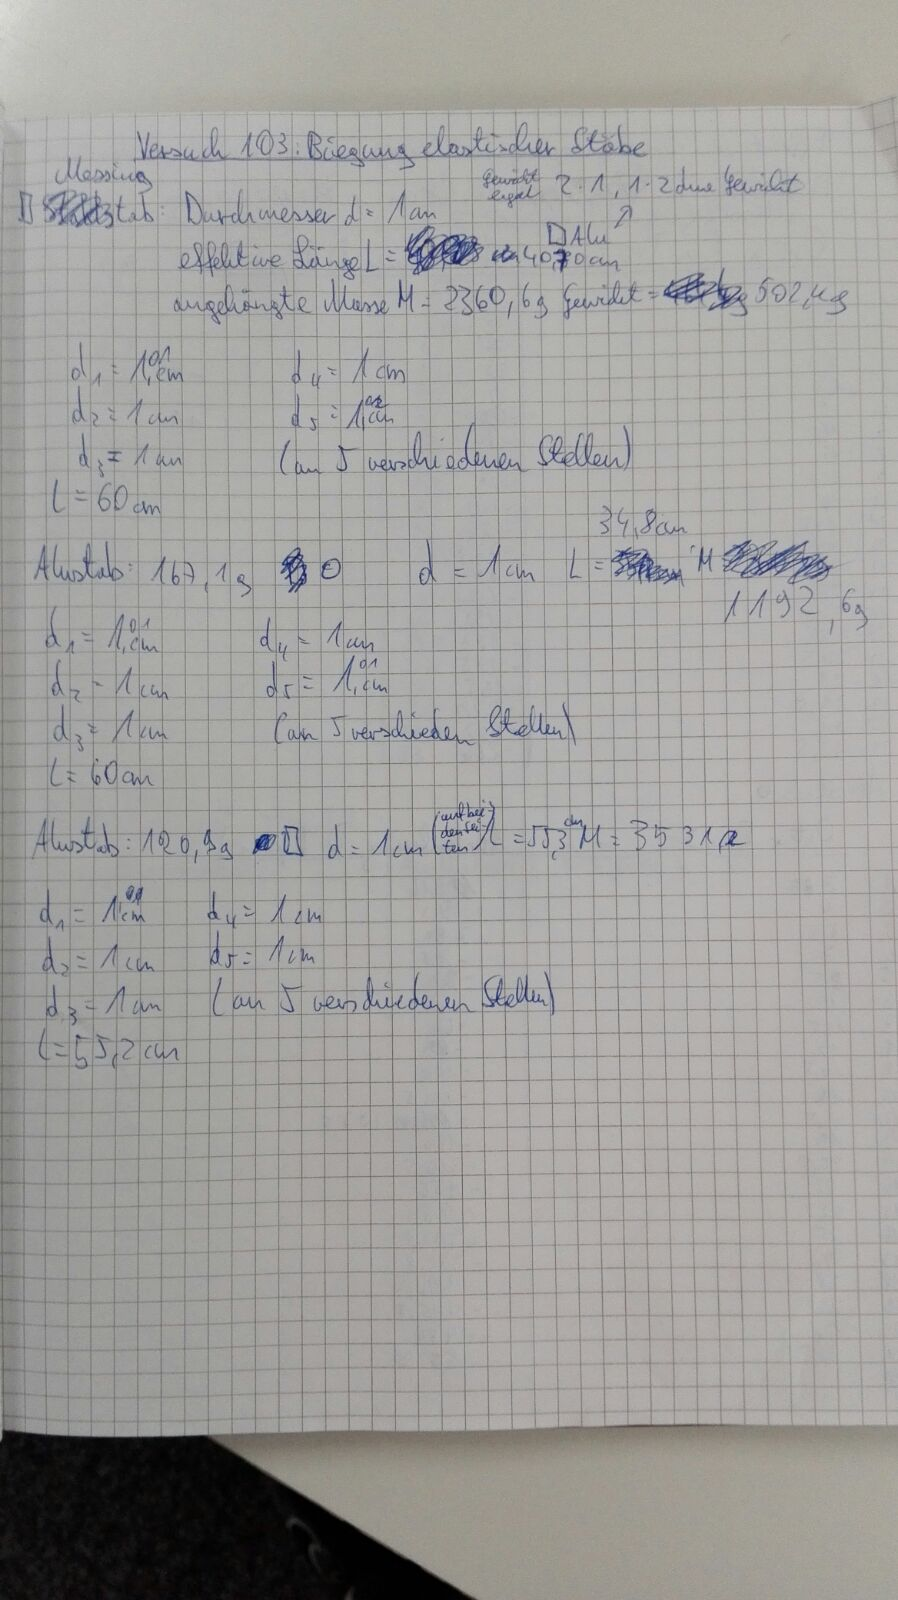
\includegraphics[width=1\textwidth]{V1034.jpeg}
    \label{fig:1034}
\end{figure}\begin{figure}[H]
    \centering
    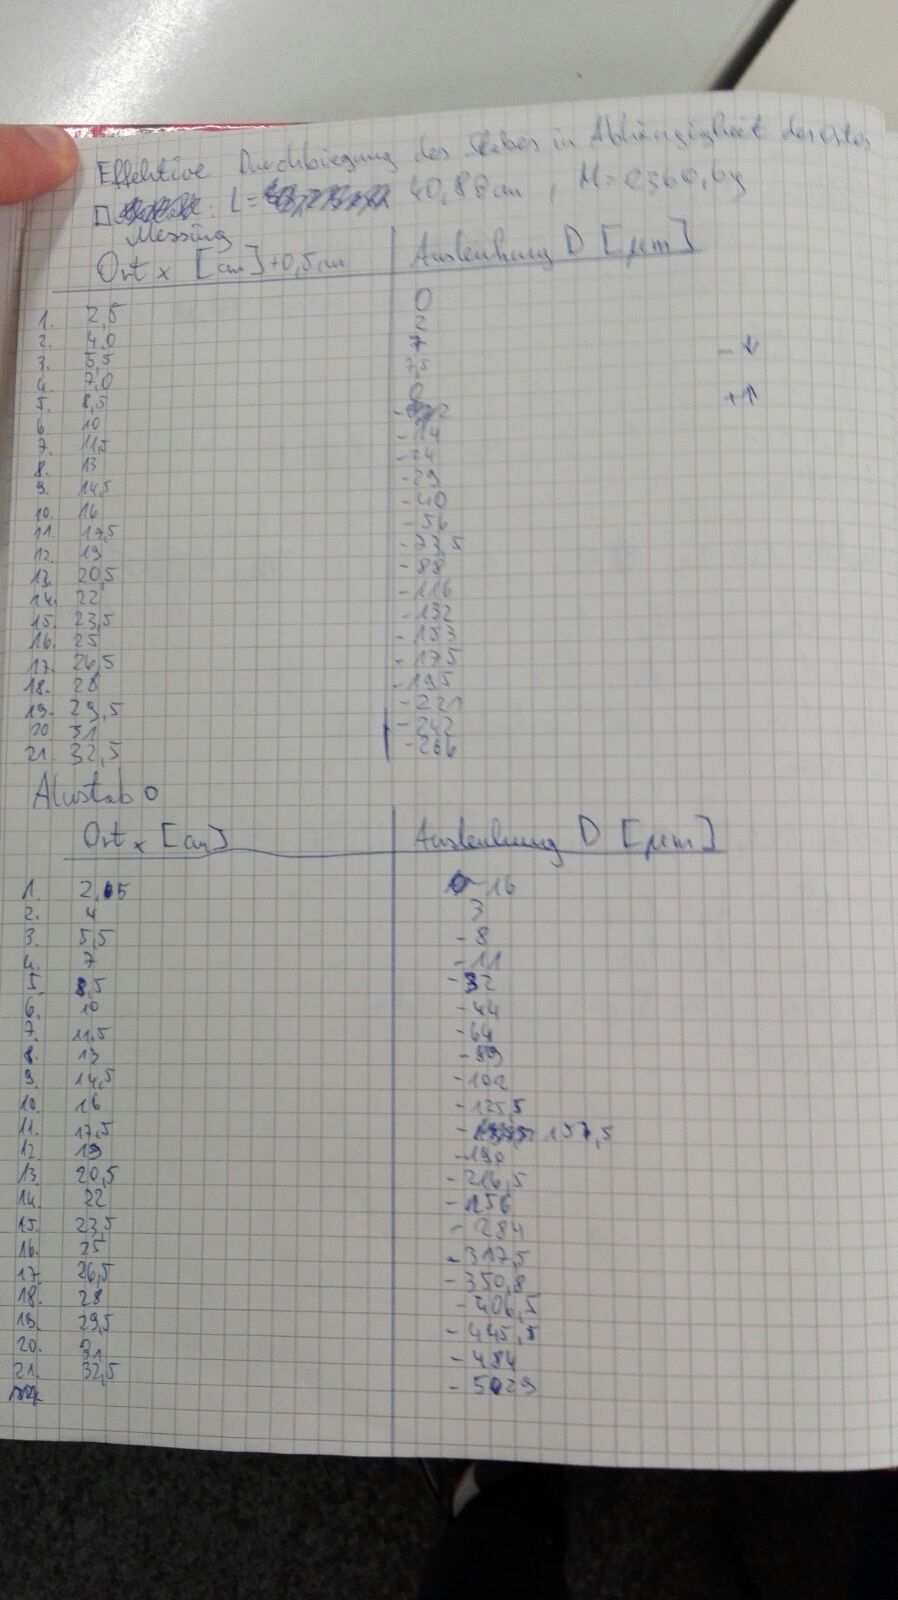
\includegraphics[width=1\textwidth]{V1035.jpeg}
    \label{fig:1035}
\end{figure}\begin{figure}[H]
    \centering
    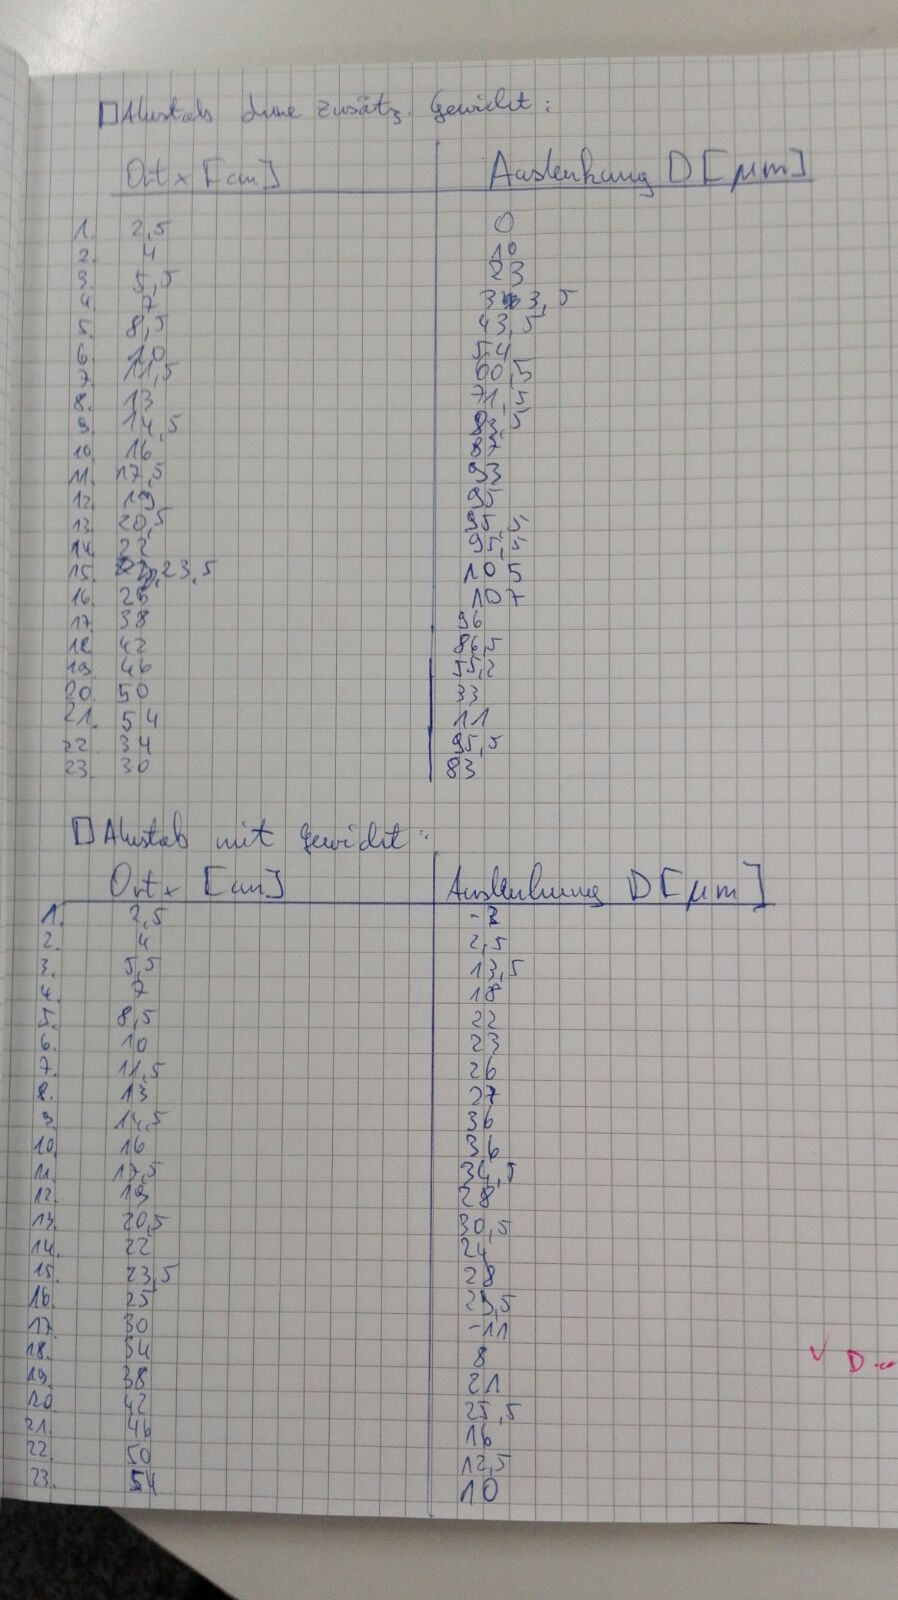
\includegraphics[width=1\textwidth]{V1036.jpeg}
    \label{fig:1036}
\end{figure}
\end{document}
